% Presentation Beamer
% Characteristics:
% -- Several Themes
% -- 

%%%%%%%%%%%%%%%%%%%%%%
%%%%%%%%%%%%%%%%%%%%%%
%%% Document Start %%%
%%%%%%%%%%%%%%%%%%%%%%
%%%%%%%%%%%%%%%%%%%%%%

\documentclass{beamer}

%%%%%%%%%%%%%%%%%%%%%%%%
%%% General Settings %%%
%%%%%%%%%%%%%%%%%%%%%%%%

%%% Packages %%%
\usepackage{verbatim}
\usepackage{graphicx}
\usepackage{subfig}
\usepackage{float}
\usepackage[ruled,linesnumbered]{algorithm2e}

%%% Definitions %%%

%%% Theme Selection %%%
%\usetheme{AnnArbor}
\usetheme{Antibes}
%\usetheme{Bergen}
%\usetheme{Berkeley}
%\usetheme{Berlin}
%\usetheme{Boadilla}
%\usetheme{boxes}
%\usetheme{CambridgeUS}
%\usetheme{Copenhagen}
%\usetheme{Darmstadt}
%\usetheme{default}
%\usetheme{Frankfurt}
%\usetheme{Goettingen}
%\usetheme{Hannover}
%\usetheme{Ilmenau}
%\usetheme{JuanLesPins}
%\usetheme{Luebeck}
%\usetheme{Madrid}
%\usetheme{Malmoe}
%\usetheme{Marburg}
%\usetheme{Montpellier}
%\usetheme{PaloAlto}
%\usetheme{Pittsburgh}
%\usetheme{Rochester}
%\usetheme{Singapore}
%\usetheme{Szeged}
%\usetheme{Warsaw}

%%% PDF Subject Catalog %%%
% - This is only inserted into the PDF information catalog. Can be left
% out.
\subject{Reinforcement Learning}

%%% Institution Logo %%% - Optional
% If you have a file called "university-logo-filename.xxx", where xxx
% is a graphic format that can be processed by latex or pdflatex,
% resp., then you can add a logo as follows:
\pgfdeclareimage[height=0.5cm]{university-logo}{university-logo-filename}
\logo{\pgfuseimage{university-logo}}

%%%%%%%%%%%%%%%%%%%%%%%%%%
%%% Presentation Cover %%%
%%%%%%%%%%%%%%%%%%%%%%%%%%

%%% Presentation Title %%%
\title{Defenses against Adversarial Examples}

%%% Subtitle %%% - Optional
%\subtitle{and Other RL Methods}

%%% Presentation Authors %%%%
% - Give the names in the same order as the appear in the paper.
% - Use the \inst{?} command only if the authors have different
%   affiliation.
\author{Keller Jordan$^1$, Rene Gutierrez$^2$, Brett Gohre$^3$}

%%% Author Affiliation %%% - Optional
% - Use the \inst command only if there are several affiliations.
% - Keep it simple, no one is interested in your street address.
\institute[University of California Santa Cruz]
{
\inst{1}%
Department of Computer Science \\
UCSC
\and
\inst{2}%
Department of Applied Mathematics \& Statistics \\
UCSC
\and
\inst{3}%
Department of Physical \& Biological Sciences \\
UCSC
}


%%% Conference Name and Information %%% - Optional
% - Either use conference name or its abbreviation.
% - Not really informative to the audience, more for people (including
%   yourself) who are reading the slides on-line
\date{CMPS290, Winter 2018}

%%% Table of Contents %%% - Optional
% Delete this, if you do not want the table of contents to pop up at
% the beginning of each subsection:
\begin{comment}
\AtBeginSubsection[]
{
\begin{frame}<beamer>{Outline}
\tableofcontents[currentsection,currentsubsection]
\end{frame}
}
\end{comment}

%%%%%%%%%%%%%%%%%%%%%%%%%%%%
%%% Presentation Content %%%
%%%%%%%%%%%%%%%%%%%%%%%%%%%%

\begin{document}
	
	%%% Title Page %%%
	\begin{frame}
		\titlepage
	\end{frame}
	
	
	%%% Outline %%% - Optional
	% - You might wish to add the option [pausesections]
	% - Section and subsections will appear in the presentation overview
	% and table of contents.
	%\begin{frame}{Outline}
	%  \tableofcontents
	%\end{frame}
	
	%%% Body %%%
	\graphicspath{{figures/}}
	
	\section*{Introduction}
	
	\section*{Optimizer Robustness}
	
	\begin{frame}{Optimizer Robustness}
		\begin{block}{Optimizers Studied}
			\begin{center}
				\begin{tabular}{ l | l | l }
					Method & SGD & EG \\ \hline
					Rule & 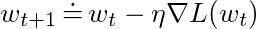
\includegraphics[width=4cm]{sgd_rule} & 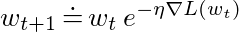
\includegraphics[width=4cm]{eg_rule}
				\end{tabular}
			\end{center}
		\end{block}
		\begin{itemize}
			\item Used extension of EG to +/- weights case for training
		\end{itemize}
	\end{frame}
	
	\begin{frame}{Procedure}
		\begin{itemize}
			\item Train FC 784-100-10 using GD and EG$\pm$ on MNIST
			\item Run untargeted adversarial attack methods
			\begin{itemize}
				\item Gradient Ascent (GA)
				\item Fast Gradient Sign (FGS)
			\end{itemize}
			\item Compare resulting models and adversarial examples
			\begin{itemize}
				\item Number of iters to fool
				\item Transferability of strong attacks
				\item Average perturbation
			\end{itemize}
		\end{itemize}
	\end{frame}
	
	\begin{frame}{Examples}
		\centering
		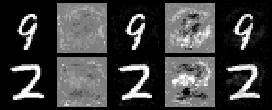
\includegraphics[width=\textwidth]{mnist_attacks}
	\end{frame}
	
	\begin{frame}{Attack Difficulty}
		\begin{block}{Number of iterations to fool network}
			\begin{center}
				\begin{tabular}{ l | l | l }
					Method / Optimizer & SGD & EG \\ \hline
					Gradient Ascent & $60.9 (\pm 32.3)$ & $85.1 (\pm 40.5)$ \\ \hline
					Fast Gradient Sign & $52.0 (\pm 26.1)$ & $91.0 (\pm 43.5)$
				\end{tabular}
			\end{center}
		\end{block}
		\begin{itemize}
			\item A network is defined as ``fooled" when its prediction changes
		\end{itemize}
	\end{frame}
	
	\begin{frame}{Average Perturbation}
		\centering
		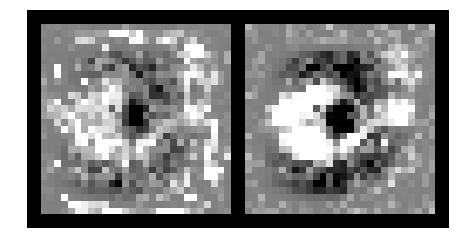
\includegraphics[width=\textwidth]{avg_attack_3}
		
		SGD (left), EG$\pm$ (right)
	\end{frame}
	
	\begin{frame}{Transferability Results}
		\begin{block}{Probability of success on other optimizer}
			\begin{center}
				\begin{tabular}{ l | l | l }
					Method / Src$\rightarrow$Dst & SGD$\rightarrow$EG & EG$\rightarrow$SGD  \\ \hline
					Gradient Ascent & 67.4\% & 99.0\% \\ \hline
					Fast Gradient Sign & 88.2\% & 99.8\%
				\end{tabular}
			\end{center}
		\end{block}
		\begin{itemize}
			\item Iterations held constant at 200 (should be comparably strong)
		\end{itemize}
	\end{frame}
	
	\begin{frame}{Results}
		\begin{itemize}
			\item Requires 1.5$\times$ stronger attacks to fool EG-trained model
			\item EG shows some robustness to attacks transferred from SGD
			\item SGD is not robust to attacks transferred to EG
			\item Attacks against EG make more sense w.r.t. expected structure of digit space
		\end{itemize}
	\end{frame}

	\section*{Reconstruction as a Defense}
	
	\begin{frame}{Defending using Reconstruction Error}
		\begin{block}{Basic idea}
			\begin{itemize}
				\item Use an architecture that reconstructs input images (CapsNet)
				\item Model will reconstruct some element of decoder-space for fooled class
				\item Adversarial images are unlikely to be in this space
				\item Expect high reconstruction error (MSE)
			\end{itemize}
		\end{block}
	\end{frame}
	
	\begin{frame}{Capsule Network Refresher}
		\centering
		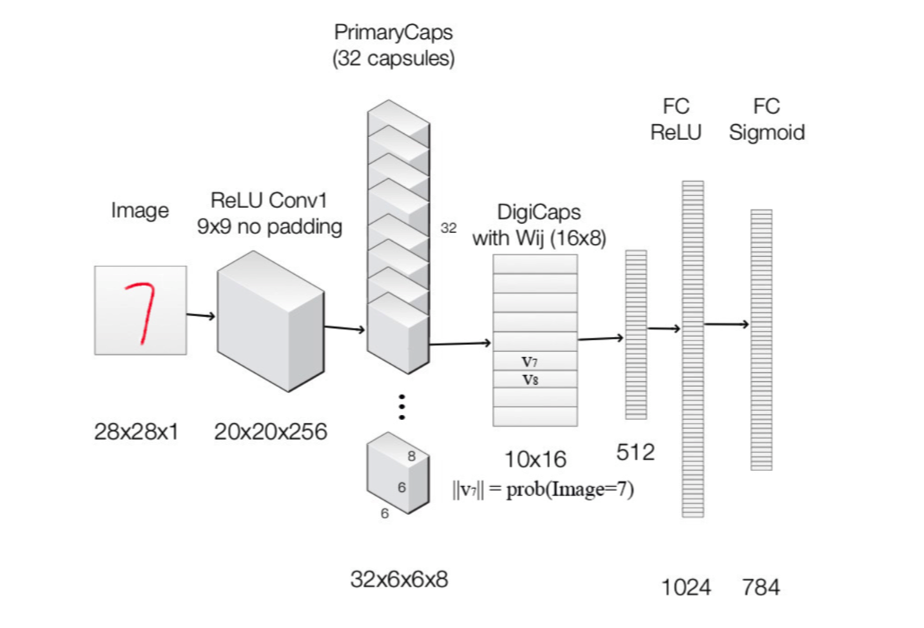
\includegraphics[width=\textwidth]{caps_recon}
	\end{frame}
	
	\begin{frame}{Reconstructions}
		\centering
		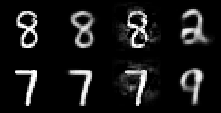
\includegraphics[width=\textwidth]{recon-fig5}
	\end{frame}
	
	\begin{frame}{Reconstructions}
		\centering
		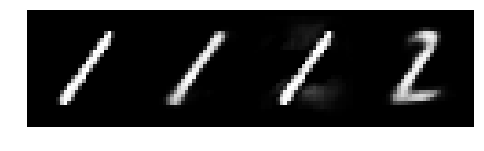
\includegraphics[width=\textwidth]{recon-fig4}		
		
		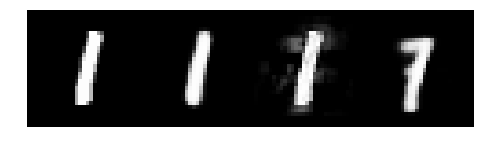
\includegraphics[width=\textwidth]{recon-fig3}
	\end{frame}
	
	\begin{frame}{Results}
		\centering
		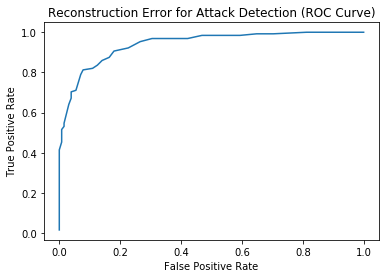
\includegraphics[width=10cm]{mse_roc}
	\end{frame}
	
	\begin{frame}{Results}
		\begin{itemize}
			\item Method successfully detects $\sim$70\% of of attacks with 5\% false-positive rate
			\item Could be improved by better loss function
			\item Unknown vulnerability to white-box attacks
			\item Expect good black-box performance due to variability of decoders and loss functions
		\end{itemize}
	\end{frame}
	
	
	% All of the following is optional and typically not needed.
	\begin{comment}
	\appendix
	\section<presentation>*{\appendixname}
	\subsection<presentation>*{For Further Reading}
	
	\begin{frame}[allowframebreaks]
	\frametitle<presentation>{For Further Reading}
	
	\begin{thebibliography}{10}
	
	\beamertemplatebookbibitems
	% Start with overview books.
	
	\bibitem{Author1990}
	A.~Author.
	\newblock {\em Handbook of Everything}.
	\newblock Some Press, 1990.
	
	
	\beamertemplatearticlebibitems
	% Followed by interesting articles. Keep the list short. 
	
	\bibitem{Someone2000}
	S.~Someone.
	\newblock On this and that.
	\newblock {\em Journal of This and That}, 2(1):50--100,
	2000.
	\end{thebibliography}
	
	\end{frame}
	
	\begin{itemize}
	\item
	Outlook
	\begin{itemize}
	\item
	Something you haven't solved.
	\item
	Something else you haven't solved.
	\end{itemize}
	\end{itemize}
	
	\end{comment}
	
\end{document}